
\documentclass[10pt,a4paper]{article}
\usepackage[utf8]{inputenc}
\usepackage{graphicx}
\usepackage{booktabs}
\title{Reporte Autom�tico de Filtros}
\date{\today}
\begin{document}
\maketitle

\section*{Resumen}
En este reporte se presentan los resultados obtenidos en el dise�o y simulaci�n de un filtro Chebyshev activo de 5 orden, con una frecuencia de corte de 10000 Hz y un ripple de $Chebyshev_3dB$.
        
\section*{Etapa 1}
R1: \textbf{896.5834564138833}\\
C1: \textbf{1e-07}\\

\noindent Arreglo resistivo recomendado:\\
R1 = 896.551724137931\texttt{||}1200.0\texttt{||}3900.0

\begin{figure}[h!]
\centering
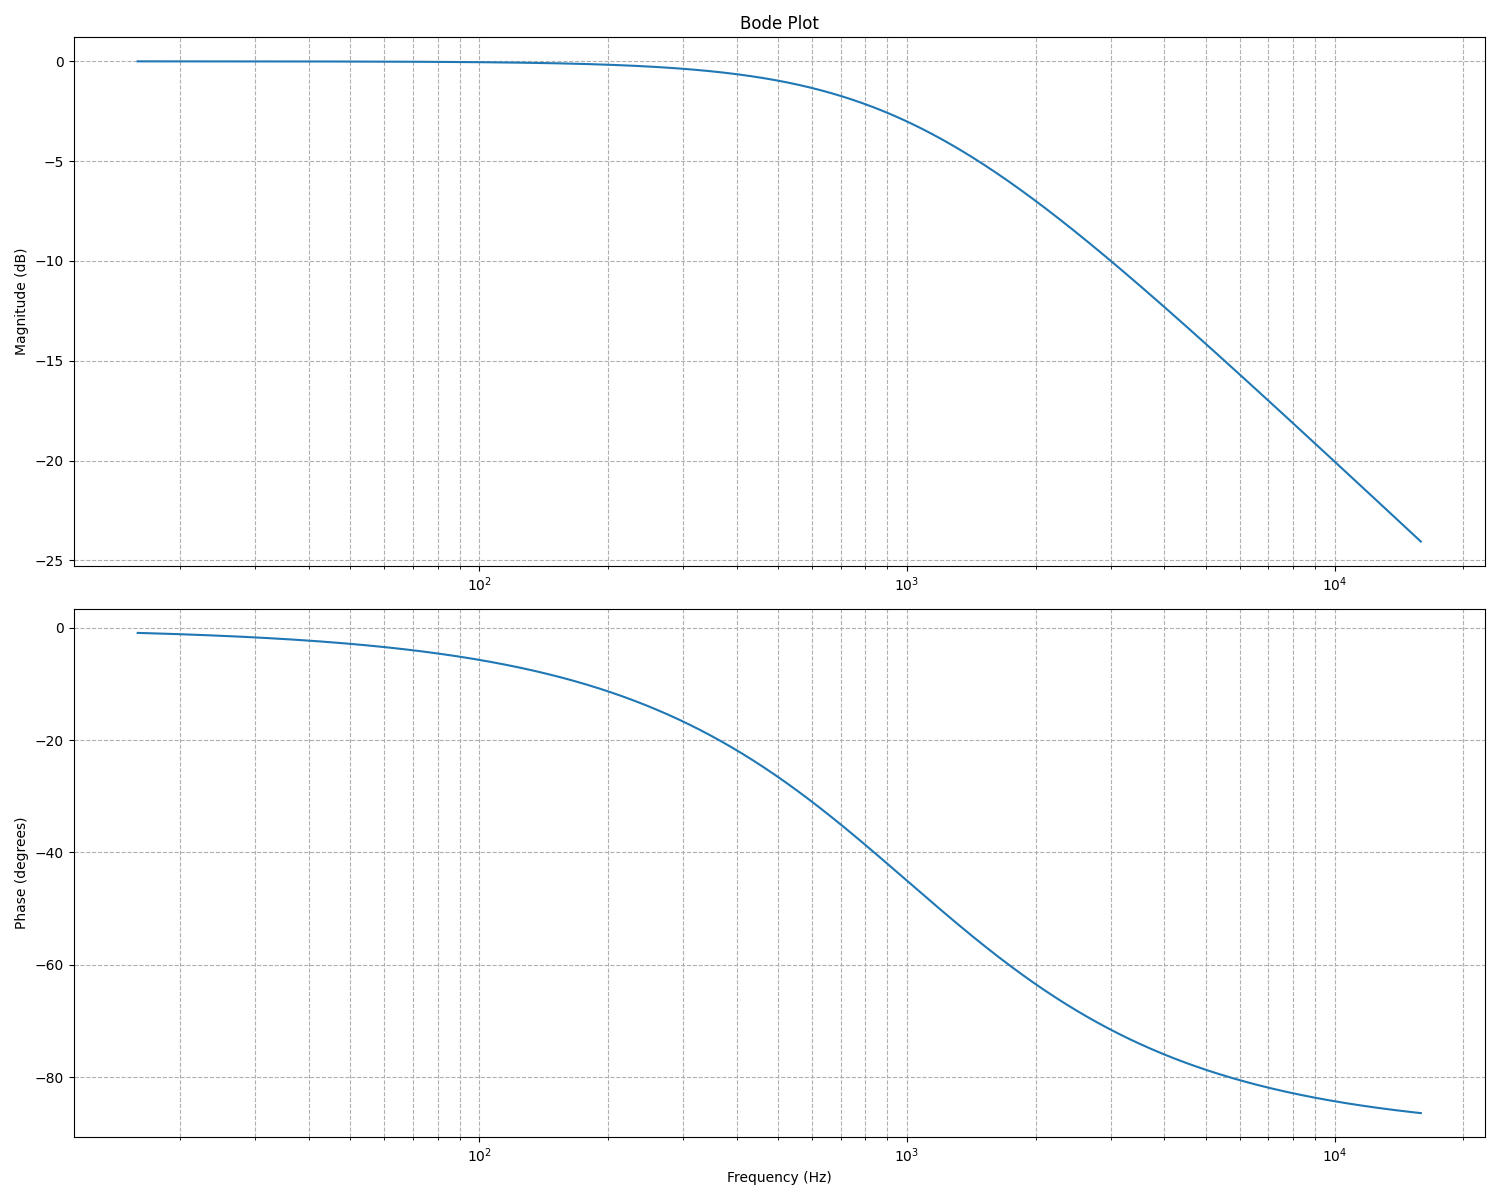
\includegraphics[width=0.8\textwidth]{bode_plot1.png}
\caption{Respuesta en frecuencia de etapa 1}
\end{figure}
        
\section*{Etapa 2}
R1: \textbf{805.6849628189005}\\
R2: \textbf{1774.6568805007644}\\
C1: \textbf{4.7e-09}\\
C2: \textbf{1e-07}\\ 


\noindent Arreglo capacitivo recomendado:\\
C2 = 1e-07+0+0\\ 

\begin{figure}[h!]
\centering
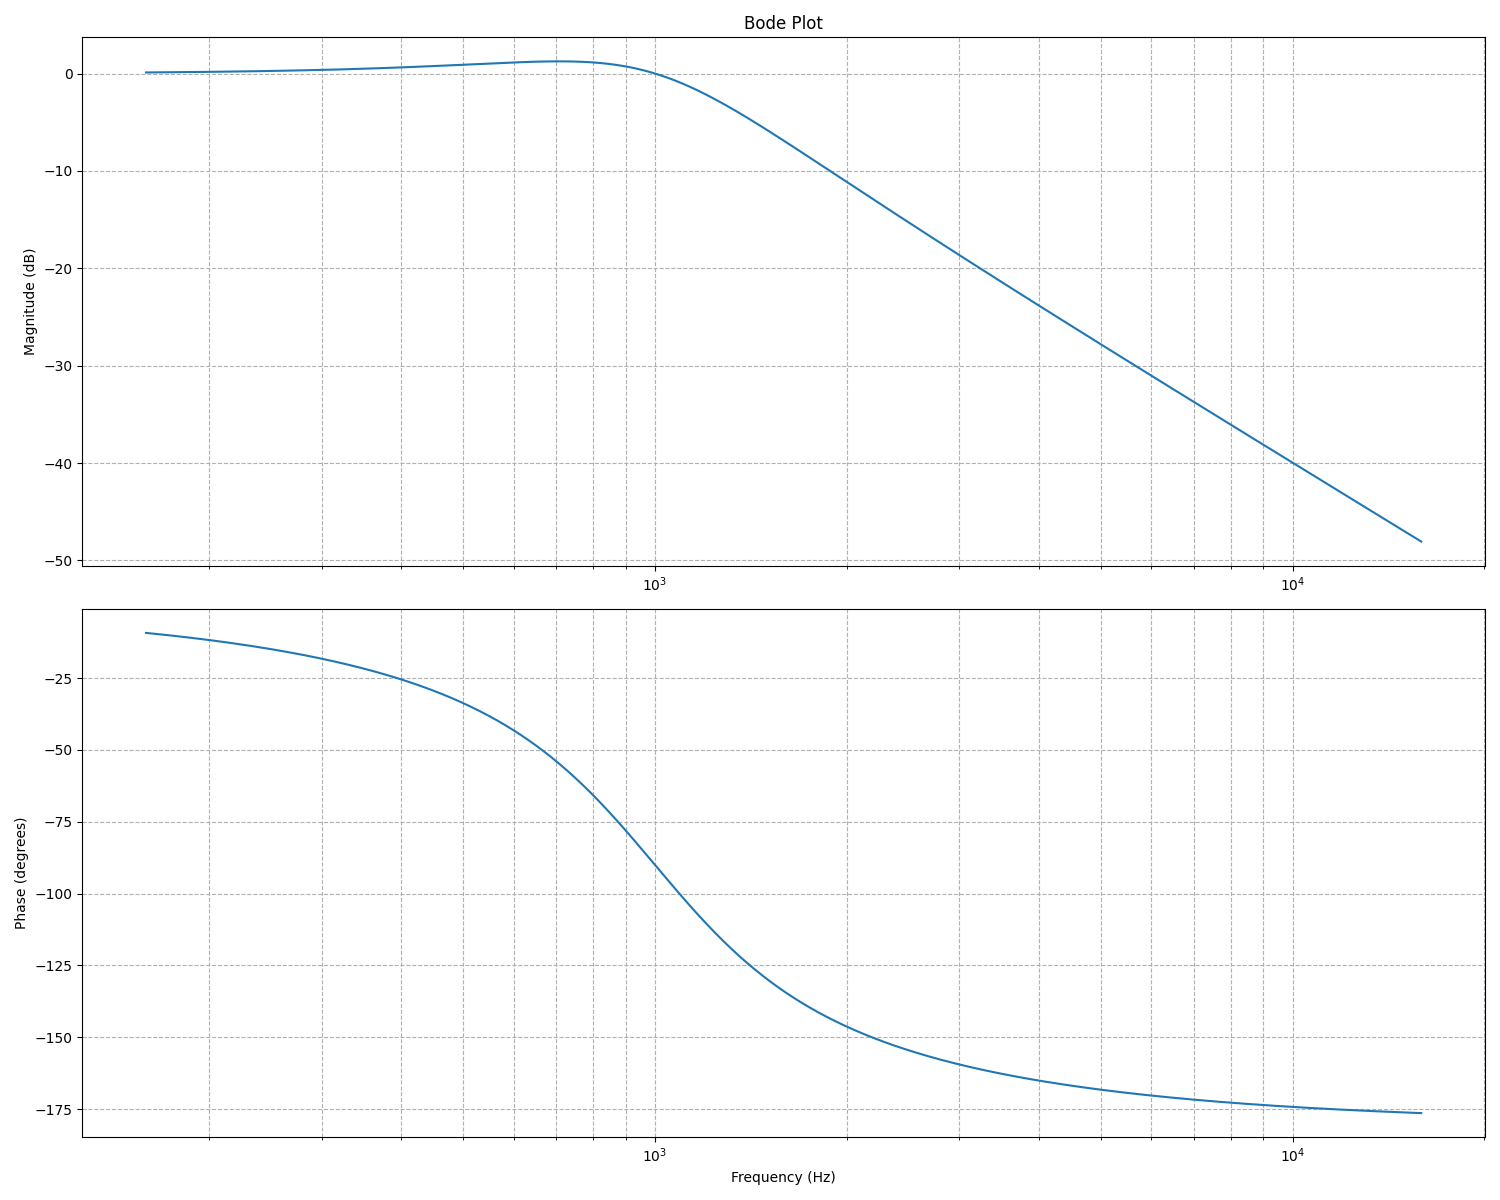
\includegraphics[width=0.8\textwidth]{bode_plot2.png}
\caption{Respuesta en frecuencia de etapa 2}
\end{figure}
        
\section*{Etapa 3}
R1: \textbf{709.9571656691953}\\
R2: \textbf{1155.3387673678176}\\
C1: \textbf{1e-09}\\
C2: \textbf{3.3e-07}\\ 


\noindent Arreglo capacitivo recomendado:\\
C2 = 4.7e-08\texttt{||}1e-07\texttt{||}2e-07\\ 

\begin{figure}[h!]
\centering
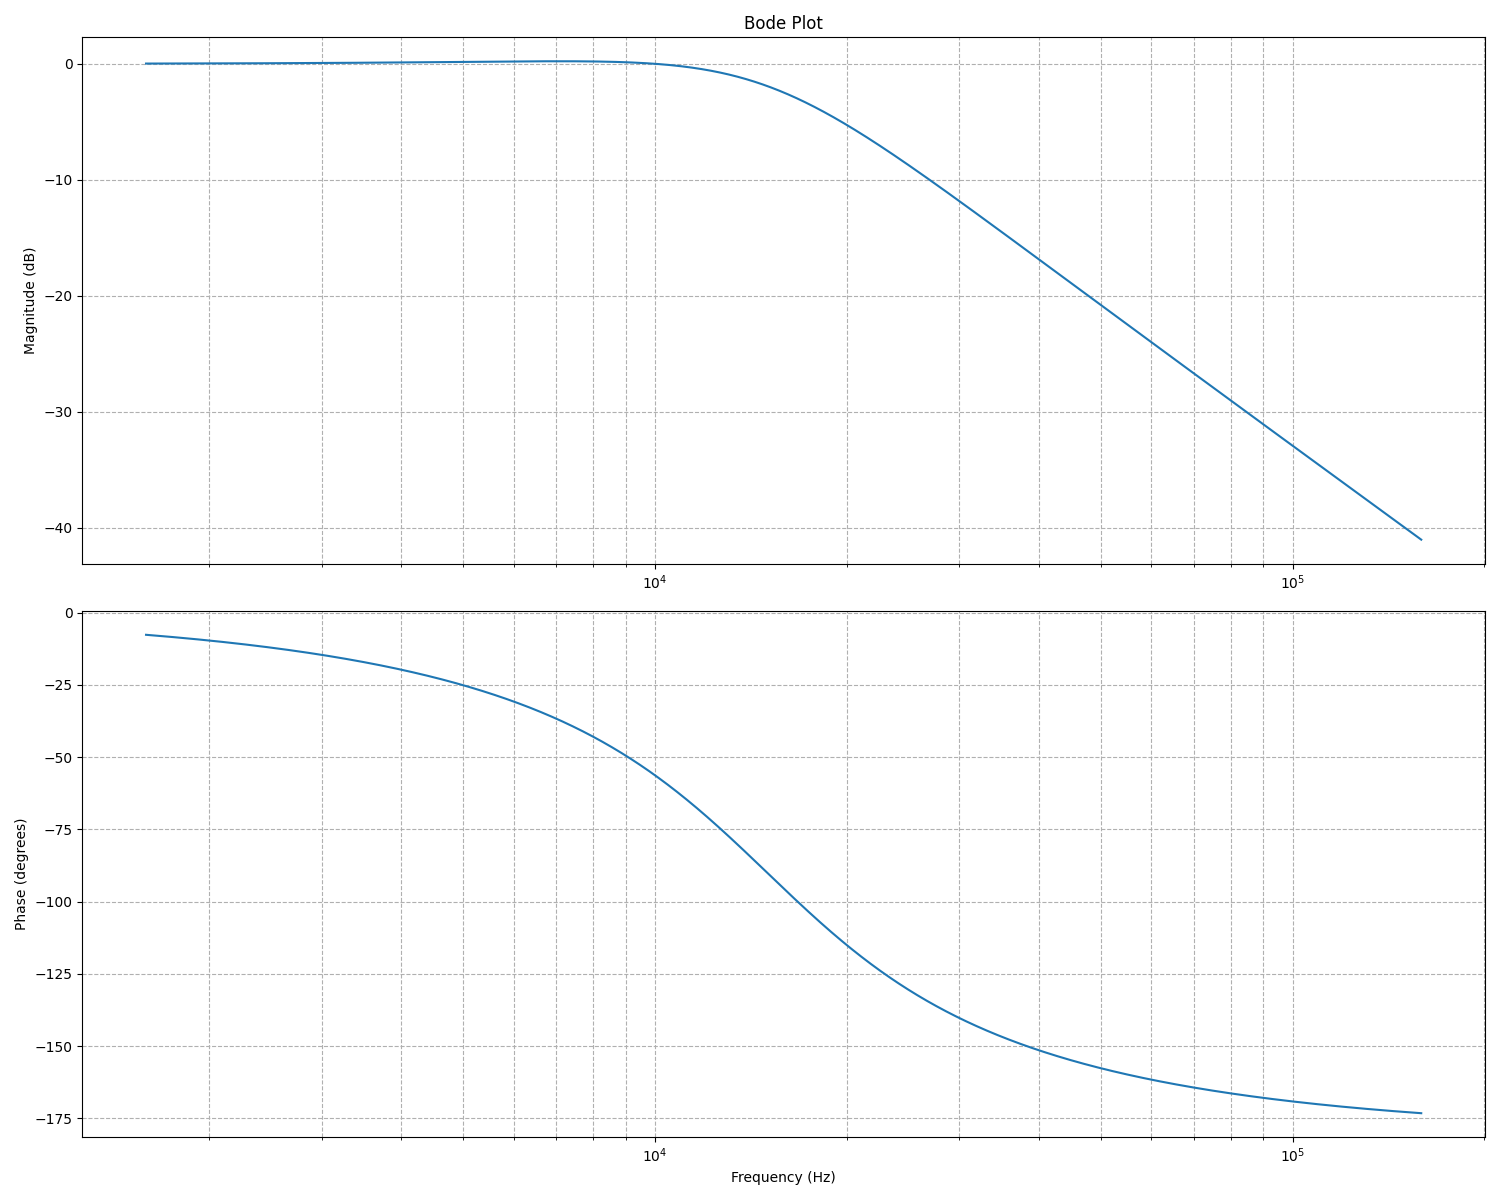
\includegraphics[width=0.8\textwidth]{bode_plot3.png}
\caption{Respuesta en frecuencia de etapa 3}
\end{figure}
        
\end{document}
